\section{Prototype methods and Nearest-Neighbours}
There exist model-free methods for classification and pattern recognition. Because they are highly unstructured, they typically are not useful for understanding the nature of the relationship between the features and class outcome but they work more in a black-box manner.

\textbf{Prototype methods} represent points in a feature space. Each prototype has an associated class label and classification of a point is made to the class of the closest prototype, generally in terms of Euclidean distance in a feature space, after each feature has been standardized (0-mean, unit variance).

\subsection{K-means clustering}
It is a method to find clusters and cluster centres in a set of unlabeled data. Once chooses the desired number of cluster centres, $R$, and the $K$-means procedure iteratively moves the centres to minimize the total within cluster variance ($K$ is the number of classes, $R$ of clusters).

Given an initial set of centres, the algorithm alternates two steps:
\begin{itemize}
\item for each centre we identify the subset of training points (its cluster) that is closer to it than any other centre;
\item the means of each feature for the data points in each cluster are computed and this mean vector becomes the new centre for that cluster.
\end{itemize}
These steps are iterated until convergence. Typically the initial $R$ centres are randomly chosen from the training set.

To use $K$-means clustering for classification of labeled data, the steps are:
\begin{itemize}
\item apply $K$-means clustering to the training data in each class separately, using $R$ prototypes;
\item assign a class label to each of the $K \times R$ prototypes;
\item classify a new feature $x$ to the class of the closest prototype.
\end{itemize}
Prototypes near the class boundaries might lead to misclassification errors for points near these boundaries. This results from the fact that for each class, the other classes do not have a say in the positioning of the prototypes for that class.

\subsection{Learning Vector Quantization}
LVQ places prototypes in strategical position w.r.t. decision boundaries. It is an online algorithm: observations are processed one at a time.

The idea is that the training points attract prototypes of the correct class, and repel other prototypes. When the iterations settle down, prototypes should be close to the training points in their class. The learning rate o$\epsilon$ is decreased to zero with each iteration. The prototypes tend to move away from the decision boundaries, and away from prototypes of competing classes.
A drawback is that they are defined by algorithms, rather than optimization of some fixed
criteria; this makes it difficult to understand their properties.
\begin{algorithm}[H]
\SetAlgoLined
Chose $R$ initial prototypes for each class: $m_1(k),\cdots, m_R(k)$, $\quad k=1,\cdots, K$, for example by sampling $R$ training points at random from each class\;
Sample a training point $(x_i, g_i)$ randomly and let $(j,k)$ index the closest prototype $m_j(k)$ to $x_i$\;
\eIf {$g_i=k$}
{
	$m_j (k) \leftarrow m_j(k) + \epsilon(x_i-m_j(k))$: move the prototype towards the the training point\;
}
{
	$m_j (k) \leftarrow m_j(k) - \epsilon(x_i-m_j(k))$: move the prototype away from the training point\;
}
Repeat step 2, decreasing the learning rate $\epsilon$ with each iteration towards $0$.
\caption{Learning Vector Quantization}
\end{algorithm}


\subsection{Gaussian Mixtures}
Each cluster is described in terms of a Gaussian density with mean and covariance matrix. The two steps of the alternating EM algorithm are very similar to the two steps in $K$-means:
\begin{itemize}
\item In the E-step, each observation is assigned a responsibility or weight for each cluster, based on the likelihood of each of the corresponding Gaussians. Observations close to the centre of a cluster will most likely get weight $1$ for that cluster, and weight $0$ for every other cluster. Observations half-way between two clusters divide their weight accordingly.
\item In the M-step, each observation contributes to the weighted means (and covariances) for every cluster.
\end{itemize}
The Gaussian mixture model is often referred to as a soft clustering method, while K-means is hard. When Gaussian mixture models are used to represent the feature density in each class, it produces smooth posterior probabilities while the classification rule is $\hat{G}(x) = \argmax{k}{\hat{p}_k(x)}$.

Although the decision boundaries are roughly similar, those for the mixture model are smoother (although the prototypes are in approximately the same positions). 

\begin{figure}
\begin{subfigure}{0.49\textwidth}
\centering
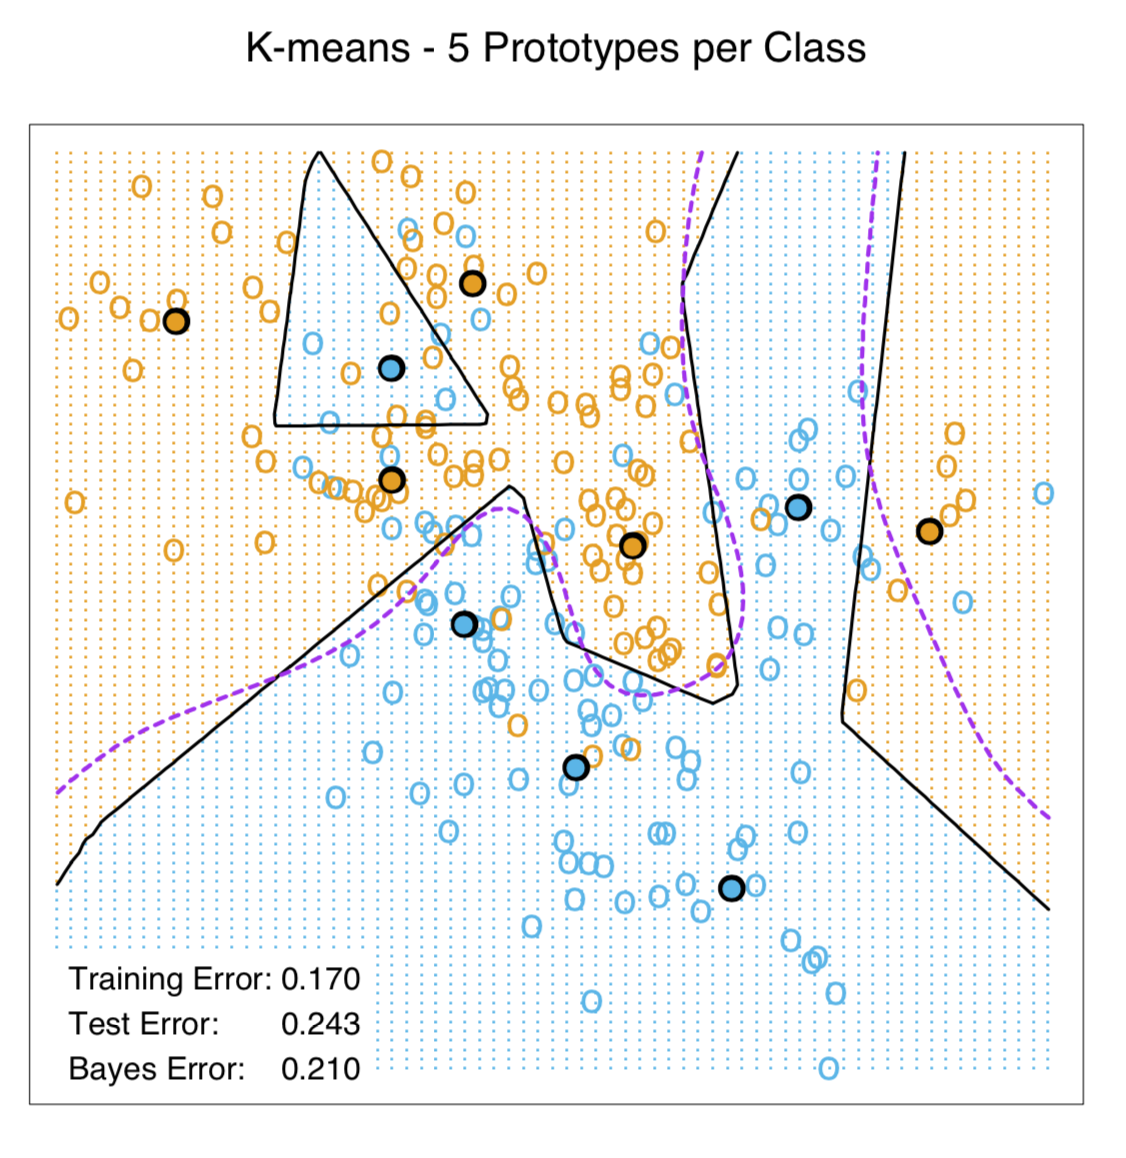
\includegraphics[width=1\linewidth]{img/kmeans}
\end{subfigure}
\hfill
\begin{subfigure}{0.49\textwidth}
\centering
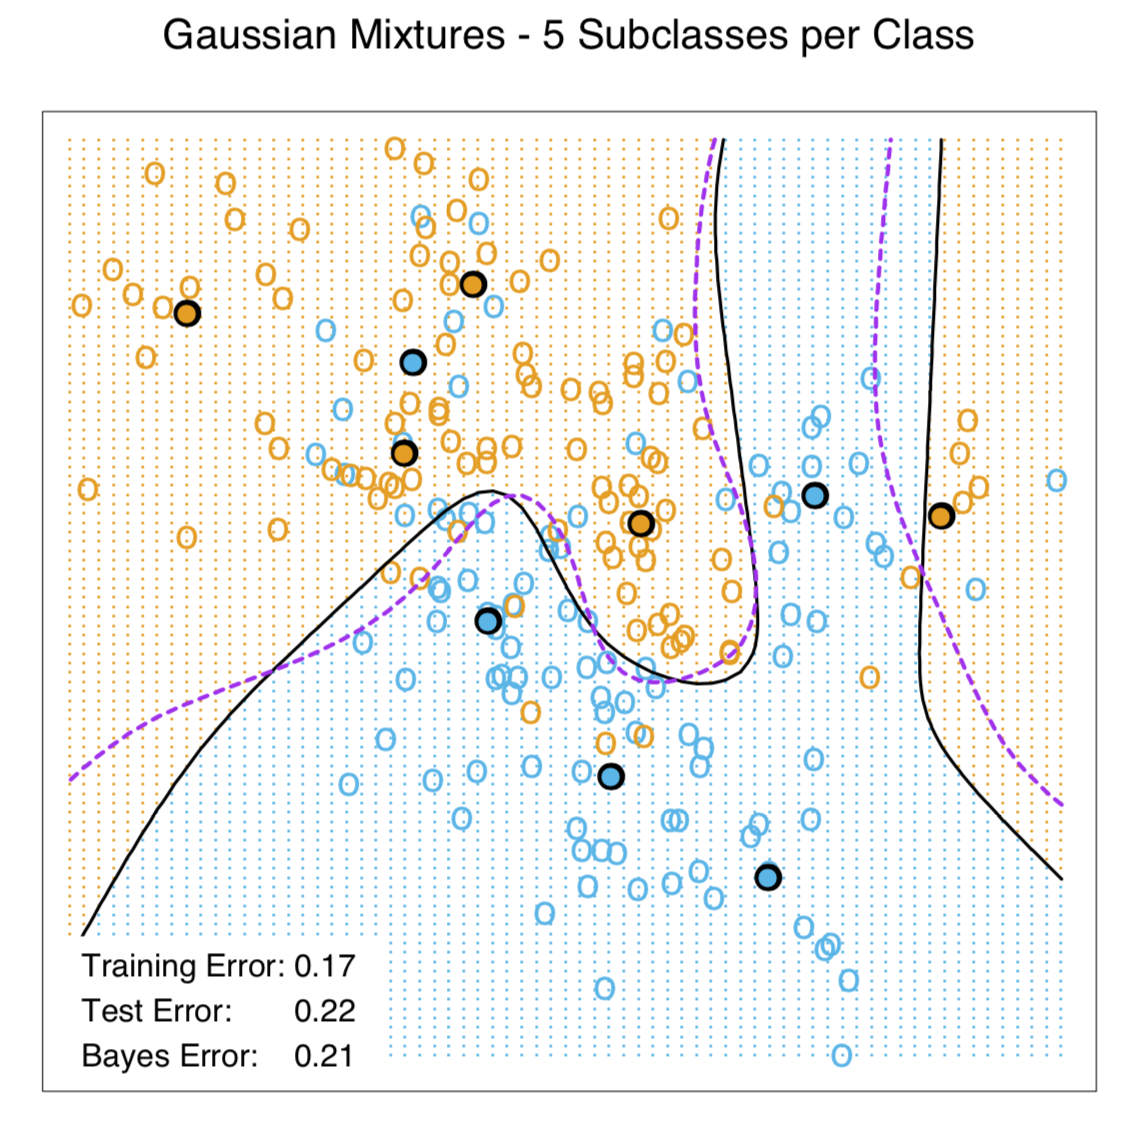
\includegraphics[width=1\linewidth]{img/GaussianMix}
\end{subfigure}
\caption{Comparison between k-means and Gaussian Mixture model with the same prototypes.}
\end{figure}

\subsection{K-nearest neighbour classifier}
These classifiers are memory-based, and require no model to be fit. Given a query point $x_0$, we find the k training points $x(r),r = 1,...,k$ closest in distance to $x_0$, and then classify using majority vote among the k-neighbours. Ties are broken at random.Typically we first standardize each of the features to have mean zero and variance 1, since it is possible that they are measured in different units. Because it uses only the training point closest to the query point, the bias of the 1-nearest-neighbour estimate is often low, but the variance is high.

\subsection{Adaptive Nearest Neighbour}
Implicit in near-neighbour classification is the assumption that the class probabilities are roughly constant in the neighbourhood, and hence simple averages give good estimates.
However, in the example of \autoref{DANN} the class probabilities vary only in the horizontal direction. If we knew this, we would stretch the neighbourhood in the vertical direction, as shown by the tall rectangular region. This will reduce the bias of our estimate and leave the variance the same.

\begin{figure}
\centering
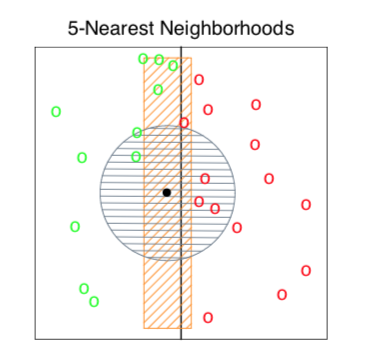
\includegraphics[scale=0.7]{img/DANN}
\caption{The points are uniform in the cube, with the vertical line separating class red and green. The vertical strip denotes the 5-nearest-neighbour region using only the horizontal coordinate to find the nearest-neighbours for the target point (solid dot). The sphere shows the 5-nearest-neighbour region using both coordinates, and we see in this case it has extended into the class-red region (and is dominated by the wrong class in this instance).}
\label{DANN}
\end{figure}

This suggests the idea of adapting metrics, so that the resulting neighbourhood stretch out in directions for which the class probabilities do not change much. One of these methods is the \textbf{Discriminant Adaptive Nearest-Neighbourhood (DANN)}. 
At each query point a neighbourhood of say 50 points is formed, and the class distribution among the points is used to decide how to deform the neighbourhood - that is, to adapt the metric. The adapted metric is then used in a nearest-neighbour rule at the query point. Thus at each query point a potentially different metric is used.

The DANN metric at a query $x_0$ is defined by:
\begin{equation}
\begin{aligned}
&D(x,x_0) = (x-x_0)^T\Sigma (x-x_0)\\
&\Sigma = \mathbf{W}^{-\frac{1}{2}} \left[ \mathbf{W}^{-\frac{1}{2}}\mathbf{B}\mathbf{W}^{-\frac{1}{2}} + \epsilon \I \right] \mathbf{W}^{-\frac{1}{2}} = \\
&\quad\quad = \mathbf{W}^{-\frac{1}{2}}\left[ \mathbf{B}^*+\epsilon\I\right] \mathbf{W}^{-\frac{1}{2}}\\
&\mathbf{W} = \sum_{k=1}^K \pi_k  \mathbf{W}_k\\
& \mathbf{B} = \sum_{k=1}^K \pi_k  (\bar{x}_k - \bar{x})(\bar{x}_k - \bar{x})^T
\end{aligned}
\end{equation}

$ \mathbf{W}$ is the pooled within-class covariance matrix and $\mathbf{B}$ is the between class covariance matrix, both computed with the $K$ nearest neighbours around $x_0$.
The formula first spheres the data with respect to $\mathbf{W}$ and then stretches the neighbourhood in the zero-eigenvalue directions of $\mathbf{B}^*$.
This makes sense, since locally the observed class means do not differ in these directions. The $\epsilon$ parameter rounds the neighbourhood, from an infinite strip to an ellipsoid, to avoid using points far away from the query point. The value of $\epsilon = 1$ seems to work well in general.

\autoref{DANNConcentr} shows the resulting neighbourhoods for a problem where the classes form two concentric circles. Notice how the neighbourhoods stretch out orthogonally to the decision boundaries when both classes are present in the neighbourhood. In the pure regions with only one class, the neighbourhoods remain circular: in these cases the between matrix $\mathbf{B} = 0$, and the $\Sigma$ is the identity matrix.
\begin{figure}
\centering
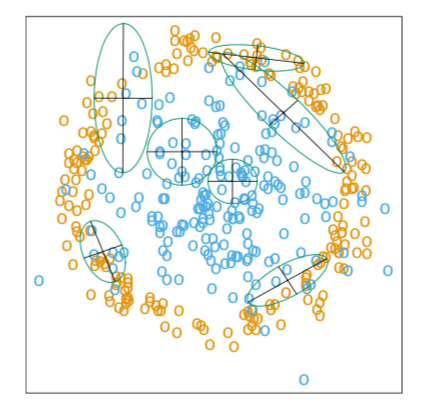
\includegraphics[scale=0.7]{img/DANNConcentr}
\caption{Neighbourhoods found by the DANN procedure, at various query points (centers of the crosses). There are two classes in the data, with one class surrounding the other. 50 nearest-neighbours were used to estimate the local metrics. Shown are the resulting metrics used to form 15-nearest-neighbourhoods.}
\label{DANNConcentr}
\end{figure}

\subsubsection{Global Dimension Reduction for Nearest Neighbours}
The discriminant-adaptive nearest-neighbour method carries out local dimension reduction, that is, dimension reduction separately at each query point. In many problems we can also benefit from global dimension reduction, that is, apply a nearest-neighbour rule in some optimally chosen subspace of the original feature space.

At each training point $x_i$, the between-centroids sum of squares matrix $\mathbf{B}_i$ is computed, and then these matrices are averaged over all training points:
\begin{equation}
\bar{\mathbf{B}} = \frac{1}{N} \sum_{i=1}^N \mathbf{B}_i
\end{equation}

Let $e_1, \cdots, e_p$ be the eigenvectors  of the matrix $\mathbf{B}$ decreasingly ordered. These eigenvectors span the optimal subspaces for global subspace reduction. The rank-$L$ approximation to $\bar{\mathbf{B}}$ is:
\begin{equation}
\bar{\mathbf{B}}_L = \sum_{\ell=1}^L \theta_\ell e_\ell e_\ell^T
\end{equation}
and it solves the least squares problem
\begin{equation}
\min_{rank(\mathbf{M}) = L} \sum_{i=1}^N trace \left[ \br{\mathbf{B}_i - \mathbf{M}}^2\right]
\end{equation}
$\mathbf{B}_i$ contains information on the local discriminant subspace and the strength of discriminant in that subsapce, it can be seen as a way of finding the best approximating subspace of dimension $L$ to a series of $N$ subspaces by weighted least squares.

For example, when some eigenvalues turn out to be large (having eigenvectors nearly spanning the interesting subspace), and the remaining six are near zero,  we project the data into the leading four-dimensional subspace, and then carry out nearest neighbour classification.

\subsubsection{Computational considerations}
One drawback of nearest-neighbour is the computational load, both in finding the neighbours and storing the entire training set.

Reducing the storage requirements is difficult, and various editing and condensing procedures have been proposed. The idea is to isolate a subset of the training set that suffices for nearest-neighbour predictions, and throw away the remaining training data. Intuitively, it seems important to keep the training points that are near the decision boundaries and on the correct side of those boundaries, while some points far from the boundaries could be discarded.
The multi-edit algorithm of Devijver and Kittler (1982) divides the data cyclically into training and test sets, computing a nearest neighbour rule on the training set and deleting test points that are misclassified. The idea is to keep homogeneous clusters of training observations.

The condensing procedure of Hart (1968) goes further, trying to keep only important exterior points of these clusters. Starting with a single randomly chosen observation as the training set, each additional data item is processed one at a time, adding it to the training set only if it is misclassified by a nearest-neighbour rule computed on the current training set.
